\documentclass{article}



\usepackage[utf8]{inputenc}
\usepackage{longtable}
\usepackage{authblk}
\usepackage{adjustbox}

\usepackage{natbib}

% autores
\title{LOS INDICES DE COLOMBIA}


\renewcommand\Authand{, y }
\author[1]{\normalsize NATALIA MEJIA}

\affil[1]{\small  Escuela de Ingeniería,Universidad de los Andes\\
\texttt{{n.mejia12}@uniandes.edu.co}}

\date{4 de Julio de 2018}





\usepackage{Sweave}
\begin{document}
\Sconcordance{concordance:ProyectoFNatiM.tex:ProyectoFNatiM.Rnw:%
1 27 1 1 0 18 1 1 7 6 1 1 5 15 0 1 2 5 1 1 8 1 4 6 1 1 7 1 3 7 1 1 6 12 %
0 1 2 1 1 1 8 13 0 1 2 1 1 1 3 1 2 1 5 1 4 31 0 1 2 6 1 1 13 1 39 3 1 1 %
29 1 2 8 1}


\maketitle


\begin{abstract}
Este es mi primer trabajo en exploracion y modelamiento de indices usando LATEX. LaTeX es un sistema de composición de textos, orientado especialmente a la creación de libros, documentos científicos y técnicos que contengan fórmulas matemáticas. LaTeX está formado por un gran conjunto de macros de TeX, escrito por Leslie Lamport en 1984, con la intención de facilitar el uso del lenguaje de composición tipográfica, TeX, creado por Donald Knuth. Es muy utilizado para la composición de artículos académicos, tesis y libros técnicos, dado que la calidad tipográfica de los documentos realizados con LaTeX es comparable a la de una editorial científica de primera línea. LaTeX es software libre bajo licencia LPPL. 
\end{abstract}



\section*{Introducción}

Un indicador social sobre un país permite ver unos hechos que allí suceden. Cada uno mide de acuerdo a sus valoraciones, y busca referenciar una situación con el fin de que se mejore. Dentro del universo de medidas que le dan cuenta al mundo de las condiciones de vida de un territorio, se destacan el Índice de Progreso Social de la organización Social Progress Imperative, cuyo origen es Oxford, en el Reino Unido, liderada por el reconocido académico Michael Green. En el ramillete de investigadores y diseñadores de cifras también está la organización estadounidense Fund For Peace, que da cuenta de realidades del planeta, en temas de seguridad y conflicto.En esos 2 indicadores y, en un proceso similar al que tuvo Colombia en el Índice de Terrorismo Global, el país ha tenido avances. En la medición del Social Progress Imperative, el territorio nacional aparece en el puesto 49 en un escalafón que clasifica a 128 países de acuerdo a la capacidad de una sociedad de satisfacer las necesidades humanas fundamentales de sus ciudadanos.
Comencemos viendo que hay en la sección \ref{univariada} en la página \pageref{univariada}.

\clearpage


\section{Exploración Univariada}\label{univariada}
\begin{abstract}
Este es mi primer trabajo en exploracion y modelamiento de indices usando LATEX. LaTeX es un sistema de composición de textos, orientado especialmente a la creación de libros, documentos científicos y técnicos que contengan fórmulas matemáticas. LaTeX está formado por un gran conjunto de macros de TeX, escrito por Leslie Lamport en 1984, con la intención de facilitar el uso del lenguaje de composición tipográfica, TeX, creado por Donald Knuth. Es muy utilizado para la composición de artículos académicos, tesis y libros técnicos, dado que la calidad tipográfica de los documentos realizados con LaTeX es comparable a la de una editorial científica de primera línea. LaTeX es software libre bajo licencia LPPL.
\end{abstract}


% Table created by stargazer v.5.2.2 by Marek Hlavac, Harvard University. E-mail: hlavac at fas.harvard.edu
% Date and time: Thu, Jul 05, 2018 - 02:52:53
\begin{table}[!htbp] \centering 
  \caption{Medidas estadísticas} 
  \label{stats} 
\begin{tabular}{@{\extracolsep{5pt}}lcc} 
\\[-1.8ex]\hline 
\hline \\[-1.8ex] 
Statistic & \multicolumn{1}{c}{N} & \multicolumn{1}{c}{Median} \\ 
\hline \\[-1.8ex] 
IDH & 32 & 0.804 \\ 
Poblacion.Cabecera & 32 & 717,197 \\ 
Poblacion.Resto & 32 & 268,111.5 \\ 
Poblacion.Total & 32 & 1,028,429 \\ 
\hline \\[-1.8ex] 
\end{tabular} 
\end{table} 
\begin{abstract}
Este es mi primer trabajo en exploracion y modelamiento de indices usando LATEX. LaTeX es un sistema de composición de textos, orientado especialmente a la creación de libros, documentos científicos y técnicos que contengan fórmulas matemáticas. LaTeX está formado por un gran conjunto de macros de TeX, escrito por Leslie Lamport en 1984, con la intención de facilitar el uso del lenguaje de composición tipográfica, TeX, creado por Donald Knuth. Es muy utilizado para la composición de artículos académicos, tesis y libros técnicos, dado que la calidad tipográfica de los documentos realizados con LaTeX es comparable a la de una editorial científica de primera línea. LaTeX es software libre bajo licencia LPPL.
\end{abstract}


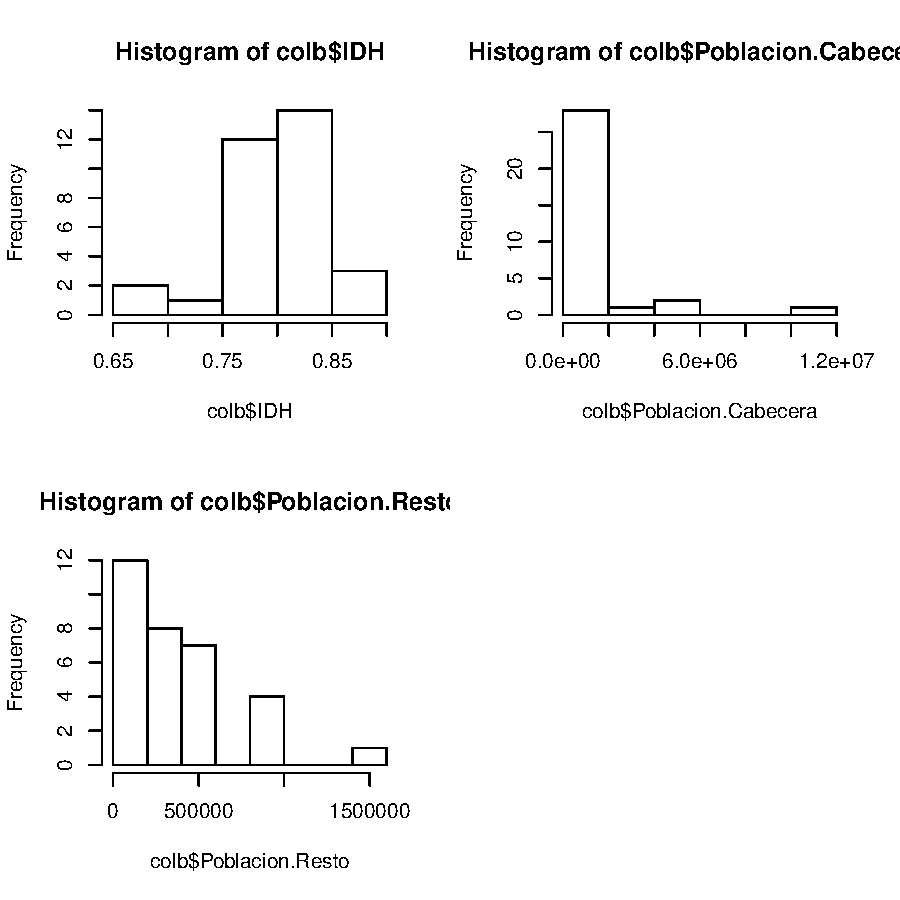
\includegraphics{ProyectoFNatiM-barplots}
\clearpage
\begin{abstract}
Este es mi primer trabajo en exploracion y modelamiento de indices usando LATEX. LaTeX es un sistema de composición de textos, orientado especialmente a la creación de libros, documentos científicos y técnicos que contengan fórmulas matemáticas. LaTeX está formado por un gran conjunto de macros de TeX, escrito por Leslie Lamport en 1984, con la intención de facilitar el uso del lenguaje de composición tipográfica, TeX, creado por Donald Knuth. Es muy utilizado para la composición de artículos académicos, tesis y libros técnicos, dado que la calidad tipográfica de los documentos realizados con LaTeX es comparable a la de una editorial científica de primera línea. LaTeX es software libre bajo licencia LPPL.
\end{abstract}



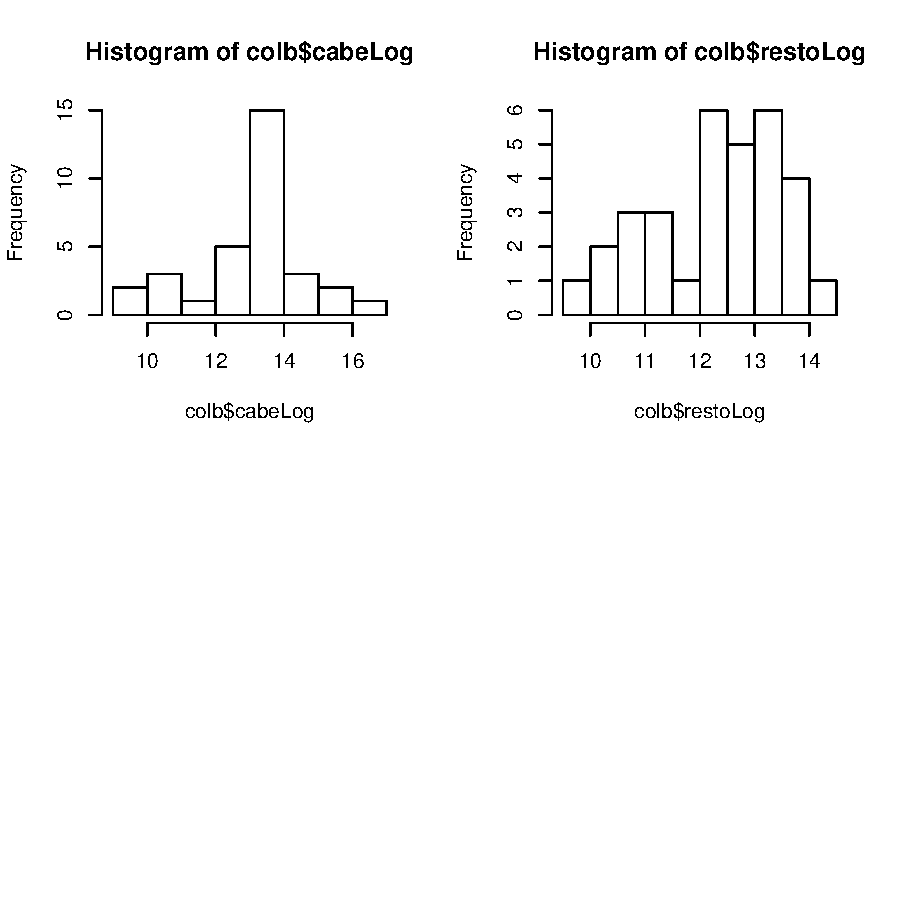
\includegraphics{ProyectoFNatiM-barplots2}
\clearpage
\section{Exploración Bivariada}\label{bivariada}
\begin{abstract}
Este es mi primer trabajo en exploracion y modelamiento de indices usando LATEX. LaTeX es un sistema de composición de textos, orientado especialmente a la creación de libros, documentos científicos y técnicos que contengan fórmulas matemáticas. LaTeX está formado por un gran conjunto de macros de TeX, escrito por Leslie Lamport en 1984, con la intención de facilitar el uso del lenguaje de composición tipográfica, TeX, creado por Donald Knuth. Es muy utilizado para la composición de artículos académicos, tesis y libros técnicos, dado que la calidad tipográfica de los documentos realizados con LaTeX es comparable a la de una editorial científica de primera línea. LaTeX es software libre bajo licencia LPPL.
\end{abstract}



% Table created by stargazer v.5.2.2 by Marek Hlavac, Harvard University. E-mail: hlavac at fas.harvard.edu
% Date and time: Thu, Jul 05, 2018 - 02:52:58
\begin{table}[!htbp] \centering 
  \caption{Correlación de Democracia con las demás variables} 
  \label{corrDem} 
\begin{tabular}{@{\extracolsep{5pt}} cc} 
\\[-1.8ex]\hline 
\hline \\[-1.8ex] 
cabeLog & restoLog \\ 
\hline \\[-1.8ex] 
$0.560$ & $0.269$ \\ 
\hline \\[-1.8ex] 
\end{tabular} 
\end{table} 

% Table created by stargazer v.5.2.2 by Marek Hlavac, Harvard University. E-mail: hlavac at fas.harvard.edu
% Date and time: Thu, Jul 05, 2018 - 02:52:58
\begin{table}[!htbp] \centering 
  \caption{correlación entre las variables independientes} 
  \label{corrDem1} 
\begin{tabular}{@{\extracolsep{5pt}} ccc} 
\\[-1.8ex]\hline 
\hline \\[-1.8ex] 
 & cabeLog & restoLog \\ 
\hline \\[-1.8ex] 
cabeLog & $1$ & $0.840$ \\ 
restoLog & $0.840$ & $1$ \\ 
\hline \\[-1.8ex] 
\end{tabular} 
\end{table} 

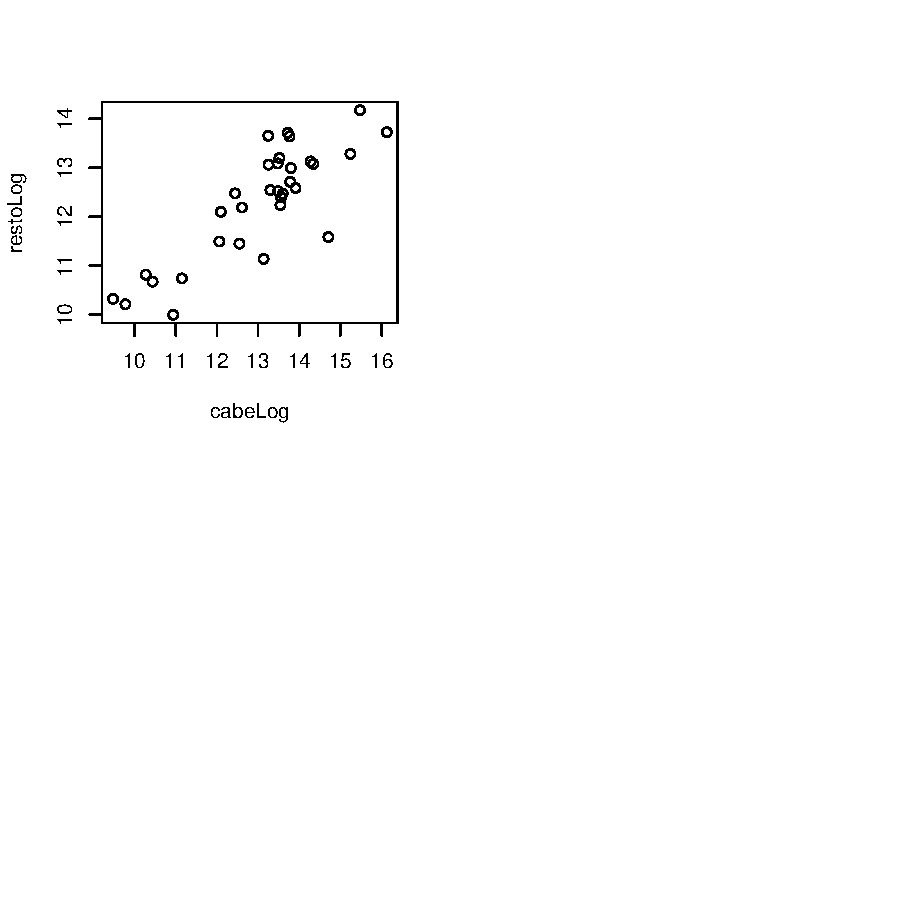
\includegraphics{ProyectoFNatiM-barplots4}


% Table created by stargazer v.5.2.2 by Marek Hlavac, Harvard University. E-mail: hlavac at fas.harvard.edu
% Date and time: Thu, Jul 05, 2018 - 02:52:58
\begin{table}[!htbp] \centering 
  \caption{Modelos de Regresión} 
  \label{regresiones} 
\begin{tabular}{@{\extracolsep{5pt}}lcc} 
\\[-1.8ex]\hline 
\hline \\[-1.8ex] 
 & \multicolumn{2}{c}{\textit{Dependent variable:}} \\ 
\cline{2-3} 
\\[-1.8ex] & \multicolumn{2}{c}{IDH} \\ 
\\[-1.8ex] & (1) & (2)\\ 
\hline \\[-1.8ex] 
 cabeLog & 0.016$^{***}$ & 0.034$^{***}$ \\ 
  & (0.004) & (0.007) \\ 
  & & \\ 
 restoLog &  & $-$0.029$^{**}$ \\ 
  &  & (0.010) \\ 
  & & \\ 
 Constant & 0.584$^{***}$ & 0.712$^{***}$ \\ 
  & (0.058) & (0.070) \\ 
  & & \\ 
\hline \\[-1.8ex] 
Observations & 32 & 32 \\ 
R$^{2}$ & 0.314 & 0.455 \\ 
Adjusted R$^{2}$ & 0.291 & 0.417 \\ 
Residual Std. Error & 0.040 (df = 30) & 0.036 (df = 29) \\ 
F Statistic & 13.701$^{***}$ (df = 1; 30) & 12.103$^{***}$ (df = 2; 29) \\ 
\hline 
\hline \\[-1.8ex] 
\textit{Note:}  & \multicolumn{2}{r}{$^{*}$p$<$0.1; $^{**}$p$<$0.05; $^{***}$p$<$0.01} \\ 
\end{tabular} 
\end{table} 

\clearpage
\section{Exploración Espacial}\label{espacial}
\begin{abstract}
Este es mi primer trabajo en exploracion y modelamiento de indices usando LATEX. Este trabajo lo he hecho bajo la filosofía de trabajo replicable. Este es mi primer trabajo en exploracion y modelamiento de indices usando LATEX. Este trabajo lo he hecho bajo la filosofía de trabajo replicable. Este es mi primer trabajo en exploracion y modelamiento de indices usando LATEX. Este trabajo lo he hecho bajo la filosofía de trabajo replicable. Este es mi primer trabajo en exploracion y modelamiento de indices usando LATEX. Este trabajo lo he hecho bajo la filosofía de trabajo replicable. \cite{gower_general_1971}
\end{abstract}



\centering

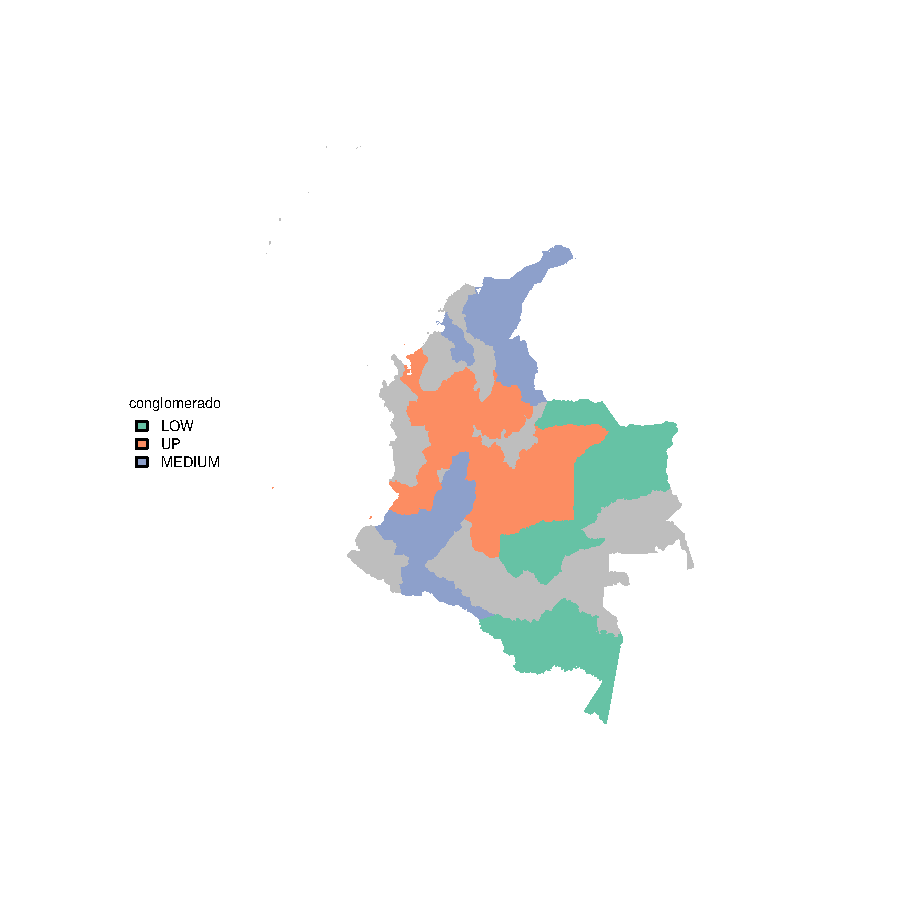
\includegraphics{ProyectoFNatiM-getMapconglomerado}

\caption{Paises conglomerados segun sus indicadores sociopolíticos}\label{clustmap}


\bibliographystyle{abbrv}
\renewcommand{\refname}{Bibliografia}
\bibliography{Colombia}

\end{document}
